\documentclass[dvisvgm,multi=true]{standalone}
\usepackage{mathmlcoresvg}
\begin{document}
%<figcaption><span>Figure 13: </span>Box model for the <code>mpadded</code> element</figcaption>
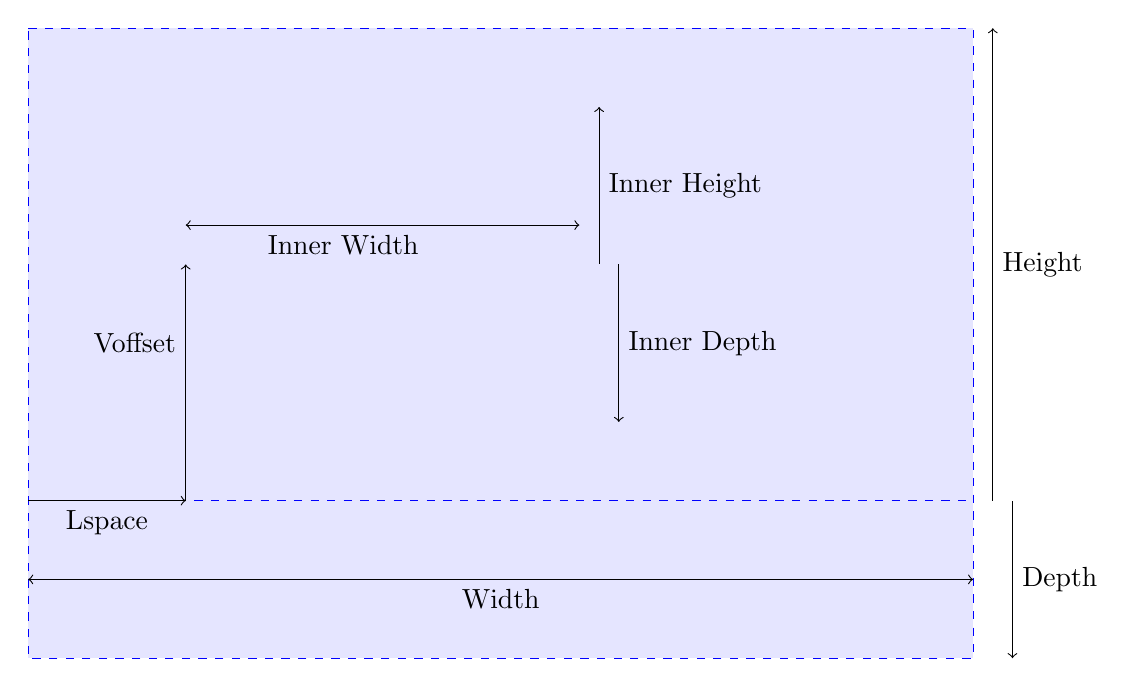
\begin{tikzpicture}[yscale=-1]
  \fill[blue!10] (0,-6) -- (12,-6) -- (12,2) -- (0,2) -- cycle;
  \draw[dashed,blue] (0,-6) -- (12,-6) -- (12,2) -- (0,2) -- cycle
  (0,0)--(12,0);

  \begin{scope}[shift={(2,-3)}]
    \MathMLBox{0}{0}{1}{1}{red}
    \draw[<->] (0,-.5) -- (2,-.5) node[below]{Inner Width} -- (5,-.5);
    \draw[<-] (5.25, -2) --
    (5.25,-1) node[right]{Inner Height} -- (5.25,0);
    \draw[<-] (5.5, 2) --
    (5.5,1) node[right]{Inner Depth} -- (5.5,0);
  \end{scope}

  \draw[<->] (0,1) -- (6,1) node[below]{Width} -- (12,1);

  \draw[<-] (12.25, -6) --
  (12.25,-3) node[right]{Height} -- (12.25,0);
  \draw[<-] (12.5, 2) --
  (12.5,1) node[right]{Depth} -- (12.5,0);

  \draw[->] (0, 0) -- (1,0) node[below]{Lspace} -- (2,0);

  \draw[->] (2, 0) -- (2,-2) node[left]{Voffset} -- (2,-3);
\end{tikzpicture}

\end{document}
